\documentclass{beamer}

% Use metropolis theme
\usepackage[progressbar=foot]{theme/beamerthememetropolis}
\usepackage{amsmath}
\usepackage{marvosym}

\title{Using Neural Networks for Time-Series Prediction}

\date{\today}
\author{Joe Jevnik}
\institute{PyData NYC 2017}

\begin{document}
\maketitle

\begin{frame}{Outline}
  \begin{itemize}
  \item<1-> Who am I?
  \item<2-> What problem did I want to solve?
  \item<3-> Data.
  \item<4-> Phrasing the problem correctly.
  \item<5-> Feature selection.
  \item<6-> Improvements.
  \end{itemize}
\end{frame}

\begin{frame}{Who am I?}
    \begin{columns}
    \column{0.5\textwidth}
    \begin{block}{Joe Jevnik}
      %\includegraphics[width=0.75\textwidth]{images/smug-mug.jpg}
    \end{block}

    \column{0.5\textwidth}
    \begin{itemize}
    \item Works at Quantopian
    \item Primarily works with storage and manipulation of time series data
    \end{itemize}
  \end{columns}
\end{frame}

\section{The Problem}

\begin{frame}{Osu!}
  \begin{itemize}
  \item<1-> Japanese rhythm game
  \item<2-> Click circles to the rhythm of music
  \item<3-> The most important time series in my life
  \end{itemize}
\end{frame}

\begin{frame}{Osu! (cont.)}
  \only<1>{
    \begin{block}{Objects}
      % 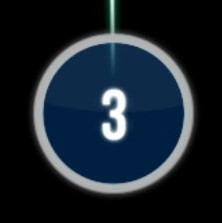
\includegraphics[width=0.75\textwidth]{circle.jpg}
      % 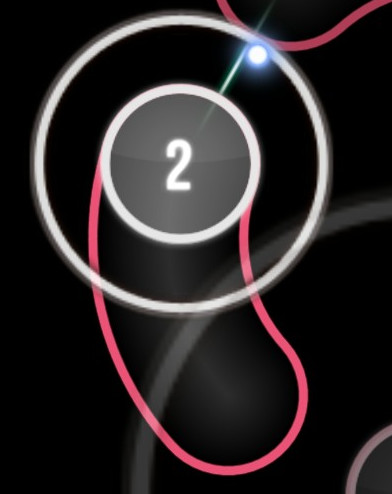
\includegraphics[width=0.75\textwidth]{slider.jpg}
    \end{block}
  }

  \only<2-5>{
    \begin{block}{Scoring}
      \begin{itemize}
      \item[]<2-> 300 points for most punctual
      \item[]<3-> 100 points for less punctual
      \item[]<3-> % \includegraphics[width=0.75\textwidth]{100.jpg}
      \item[]<4-> 50 points for least punctual
      \item[]<4-> % \includegraphics[width=0.75\textwidth]{50.jpg}
      \item[]<5-> 0 points for missing entirely
      \item[]<5-> % \includegraphics[width=0.75\textwidth]{miss.jpg}
      \end{itemize}
    \end{block}
  }

  \only<6-8>{
    \begin{block}{Sample}
      \begin{itemize}
      \item<6-> Easy
      \item<7-> Intermediate
      \item<8-> Hard
      \end{itemize}
    \end{block}

    \only<9-11>{
      \begin{block}{Mods}
        \begin{itemize}
        \item<9-> Hidden (HD)
        \item<10-> Hard Rock (HR)
        \item<11-> Double Time (DT)
        \end{itemize}
      \end{block}
    }
  }
\end{frame}

\begin{frame}{Problem}
  \begin{block}{Predict my score on a beatmap}
    \begin{itemize}
    \item[]<1-> Thousands of beatmaps
    \item[]<2-> 24 hours in a day
    \item[]<3-> Existing tools were not accurate enough
    \end{itemize}
  \end{block}
\end{frame}

\section{Data Collection}

\begin{frame}{Beatmap}
  \begin{itemize}
  \item[]<1-> Sequence of hit objects in (x, y, time) space.
  \item[]<2-> Circle Size (CS)
  \item[]<3-> Approach Rate (AR)
  \item[]<4-> Score thresholds (OD)
  \end{itemize}
\end{frame}

\begin{frame}{Replay}
  \only<1-3>{
    \begin{block}{Time series of...}
      \begin{itemize}
      \item[]<2-> Cursor location
      \item[]<3-> Keyboard state
      \end{itemize}
    \end{block}
  }

  \only<4>{
    I had about seven years of replays laying around!
  }
\end{frame}

\section{Phrasing the Problem}

\begin{frame}{Machine Learning Models}
  \only<1>{
    \begin{block}{Classifiers}
      Labels a record as a member of of a finite set of classes.
    \end{block}
  }
  \only<2>{
    \begin{block}{Regressors}
      Approximates a numerical function over the reals (IEEE floating point)
    \end{block}
  }
\end{frame}

\begin{frame}{Our Problem}
  \only<1-2>{
    \begin{block}{Classifier}
      \begin{itemize}
      \item[] 300
      \item[] 100
      \item[] 50
      \item[] 0 (miss)
      \end{itemize}
    \end{block}
    \only<2>{
      Different CS and OD mess this up.
    }
  }

  \only<3-5>{
    \begin{block}{Regressor}
      \begin{itemize}
      \item[]<3-> Predict some error metric for each hit object.
      \item[]<4-> Aim Error
      \item[]<5-> Accuracy Error
      \end{itemize}
    \end{block}
  }
\end{frame}

\begin{frame}{Error}
  \only<1-4>{
    \begin{block}{Joining Data}
      \begin{itemize}
      \item[]<1-> Find all clicks by taking times where key state changes
      \item[]<2-> Match click with the nearest hit object (ignores hit locking!)
      \item[]<3-> Compute absolute difference in time
      \item[]<4-> Compute Cartesian distance between click and circle center
      \end{itemize}
    \end{block}
  }

  \only<5-6>{
    \begin{block}{Accuracy Error}
      \begin{itemize}
      \item[]<5-> Absolute difference in time.
      \item[]<6-> Comparable across different OD
      \end{itemize}
    \end{block}
  }

  \only<7-8>{
    \begin{block}{Aim Error}
      \begin{itemize}
      \item[]<7-> Cartesian distance between click and center of circle.
      \item[]<8-> Comparable across different CS
      \end{itemize}
    \end{block}
  }

\end{document}
